\section{Brainstorming}

Im Rahmen des Projekts wird anhand des stationären Blitzers am Anckelmannsplatz (Hamburg, Deutschland) eine mögliche Arbeitsumgebung erarbeitet.

\begin{figure}[h]
\centering
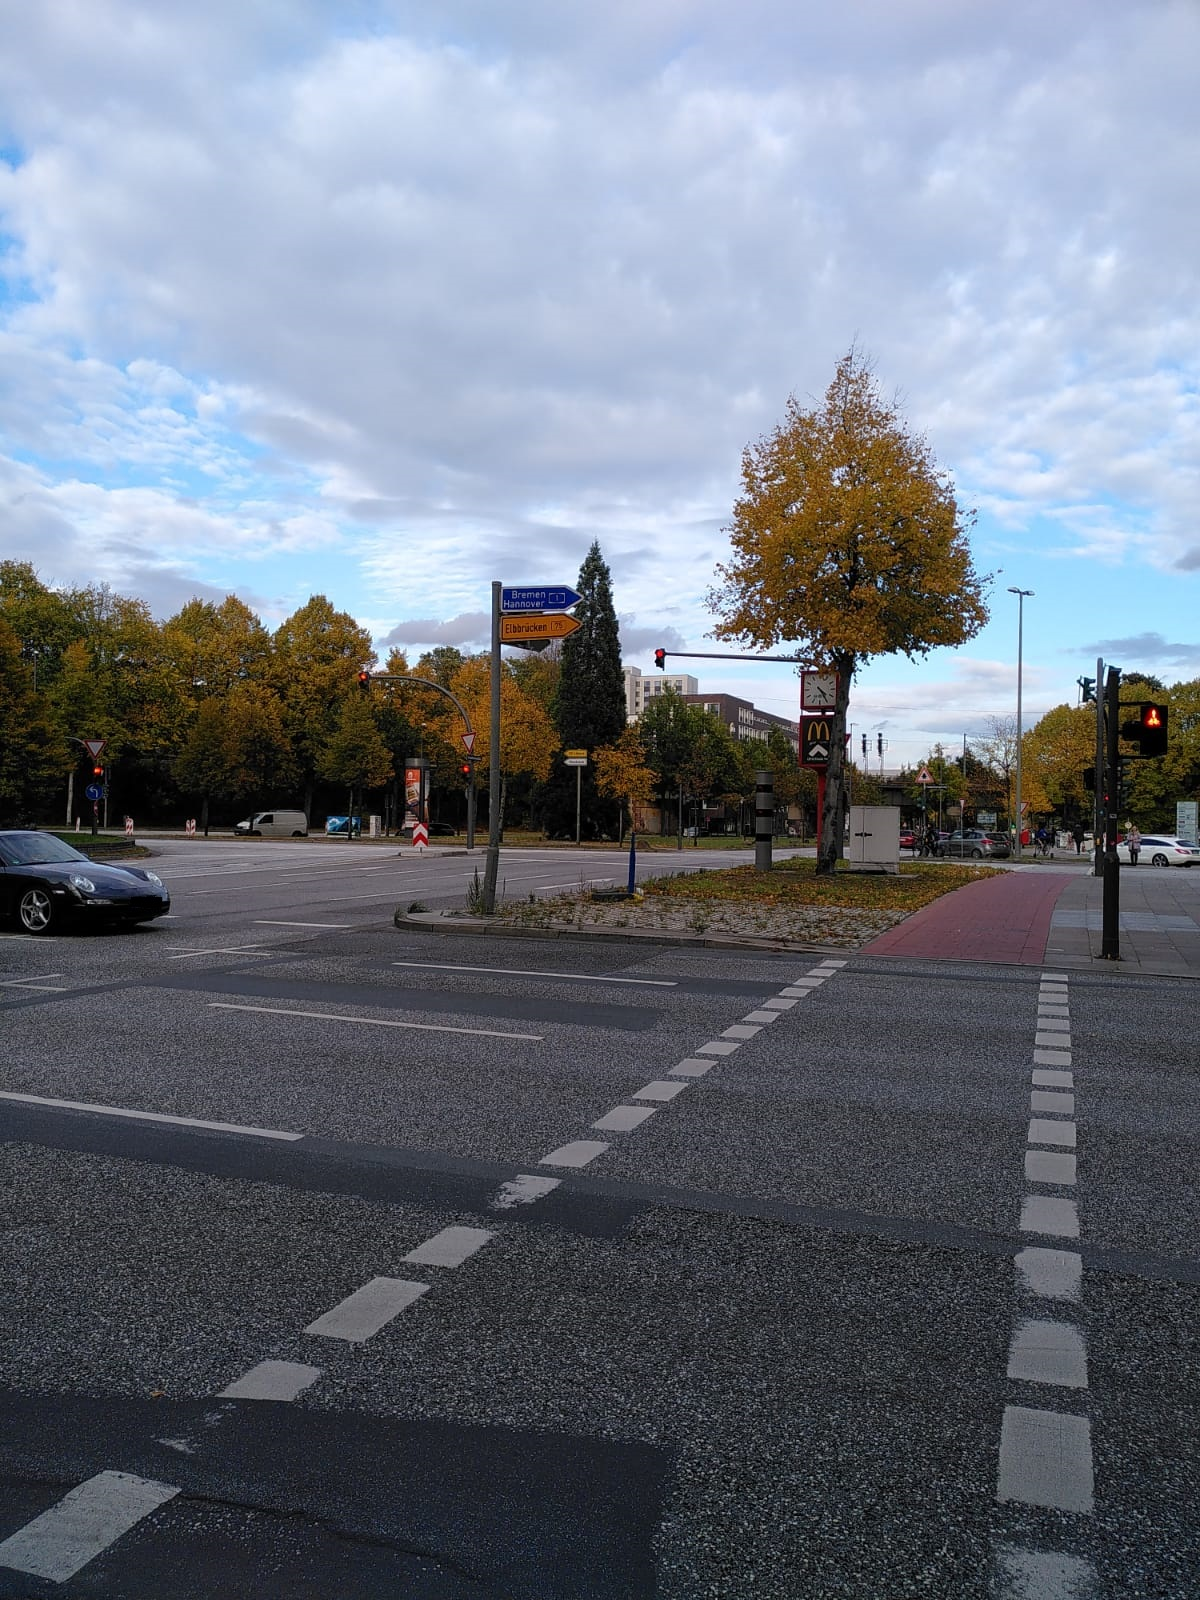
\includegraphics[scale=0.2]{Sections/Brainstorming/Blitzer.jpeg}
\caption{Blitzer Anckelmannsplatz}
\label{fig:Blitzer_Anckelmannsplatz}
\end{figure}

\begin{figure}[h]
\centering
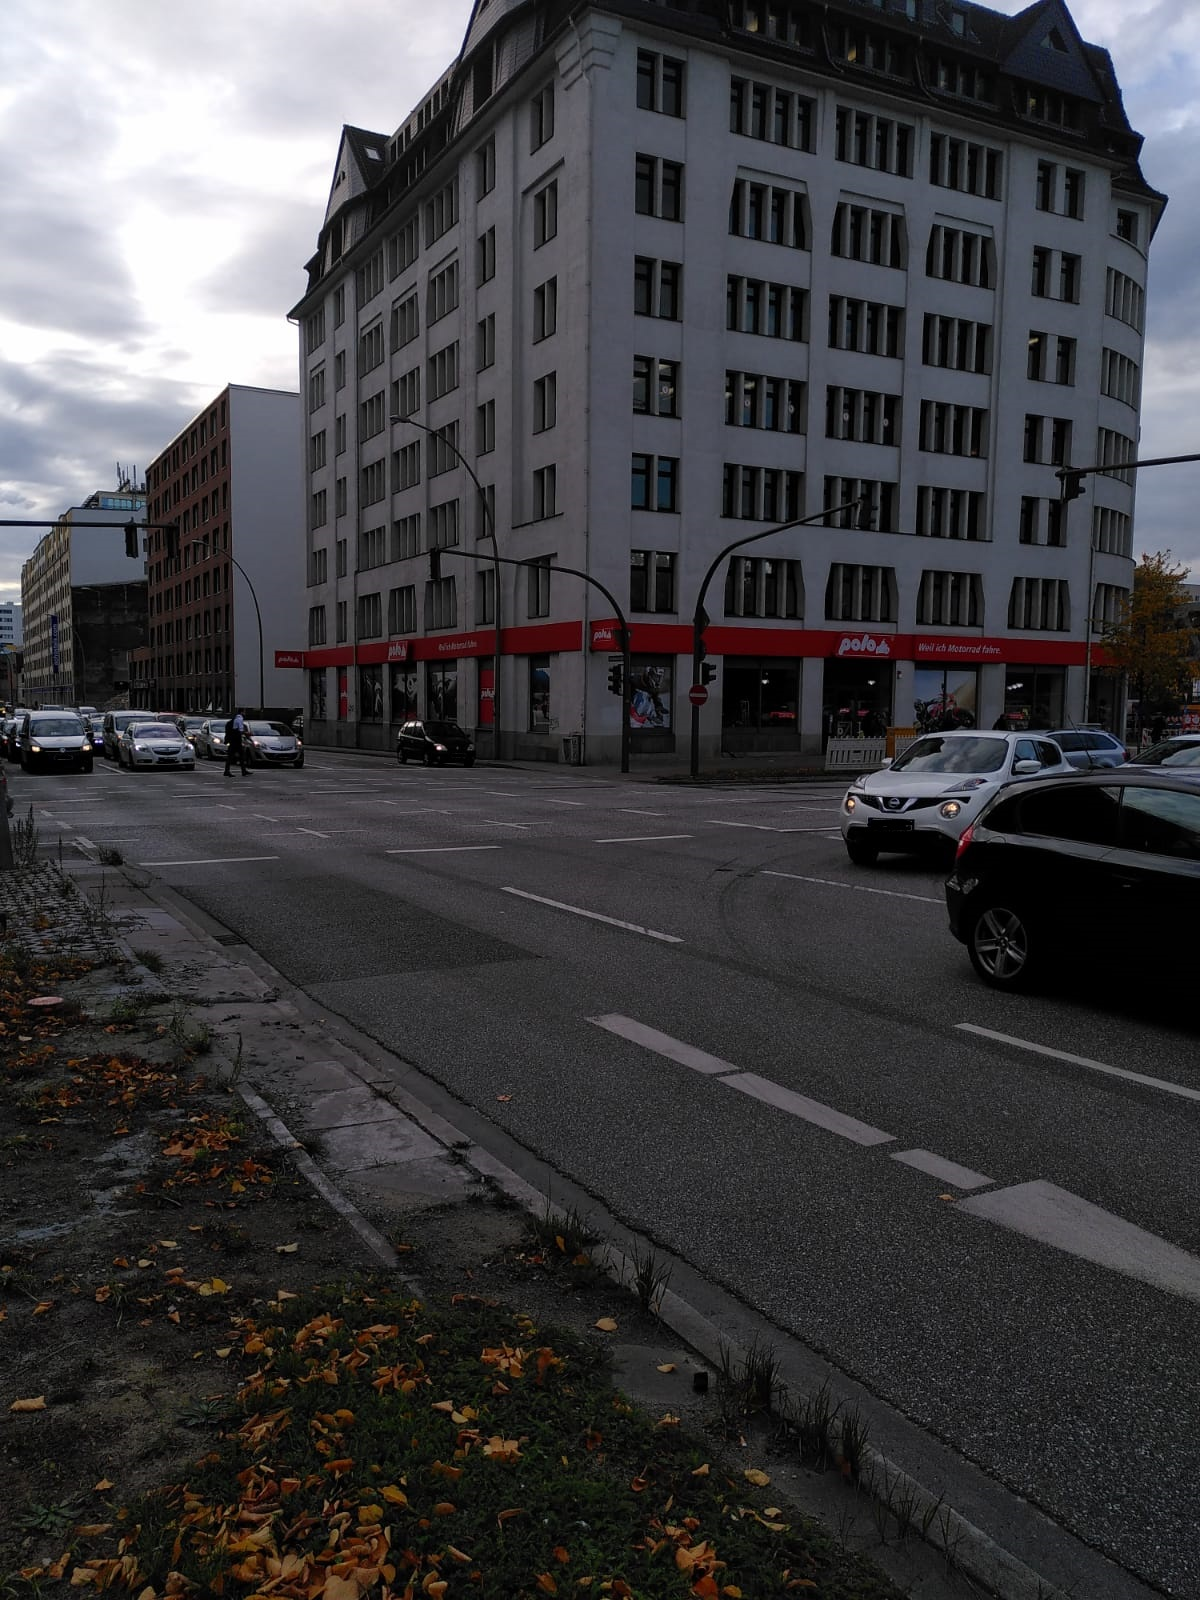
\includegraphics[scale=0.2]{Sections/Brainstorming/Blickwinkel_Blitzer_2.jpeg}
\caption{Blitzer Blickwinkel}
\label{fig:Blitzer_Blickwinkel}
\end{figure}

\newpage

\begin{figure}[h]
\centering
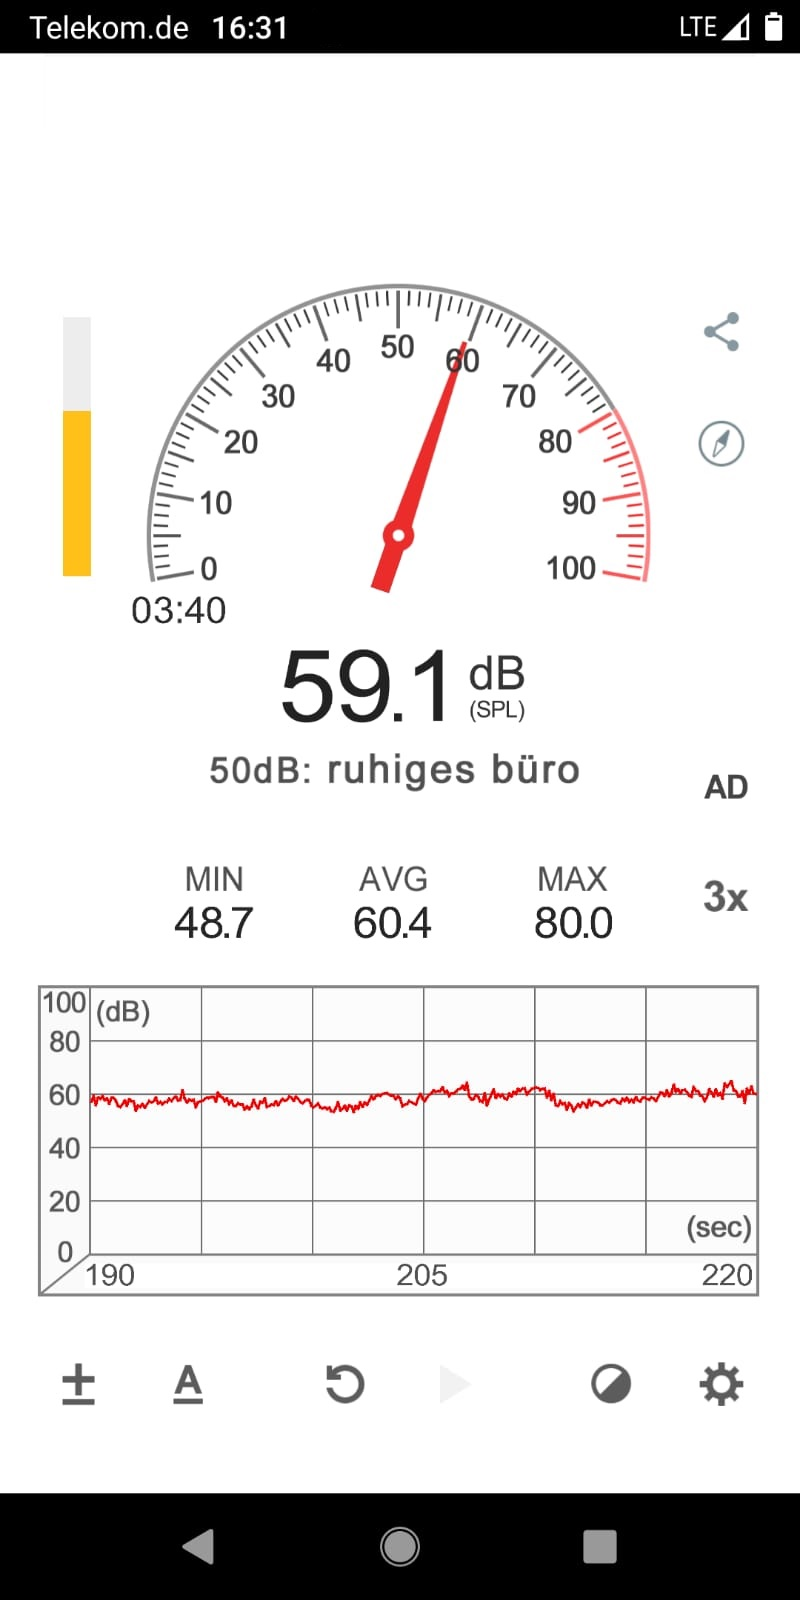
\includegraphics[scale=0.15]{Sections/Brainstorming/Pegelmessung_Anckelmannsplatz_am_Blitzer_Nachmittag.jpeg}
\caption{Schallmessung}
\label{fig:Schallmessung}
\end{figure}

Bild \ref{fig:Blitzer_Anckelmannsplatz} und \ref{fig:Blitzer_Blickwinkel} zeigen den oben genannten Blitzer, sowie den anzunehmenden Blinkwinkel. Öffnungswinkel des Detectors müssen noch erörtert werden. \\
\noindent Bild \ref{fig:Schallmessung} zeigt eine Schallmessung an einem gewöhnlichen Donnerstagnachmittag auf dem Anckelmannsplatz Höhe des Blitzers als Referenz des Pegelwertes.

\newpage

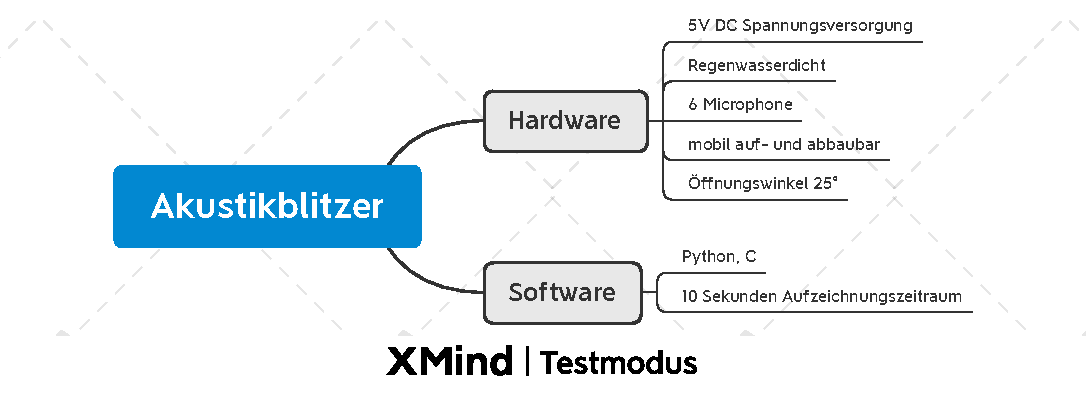
\includepdf[pages=-]{Sections/Brainstorming/2020-10-15_Brainstorming}

\newpage